\chapter{}
Como filha mais velha de um casamento problemático, com fama de sensata e precocemente amadurecida, assumi, durante a adolescência, o papel de algodão entre cristais para amenizar o clima em casa.
Não por delegação de alguém, mas porque é sempre o que acaba naturalmente acontecendo.
Só que isto ficou muito pesado e, a partir de certo tempo, intuí que inútil, também.
Comecei a achar até que quanto mais depressa meus pais se vissem sozinhos, maior seria a possibilidade de eles recomporem sua relação.
Esse era um dos motivos de eu não querer voltar a morar em casa.
O outro, só vim a compreender com clareza muito mais tarde, e nada tinha a ver com a situação familiar, ao menos não diretamente – era a minha inconformidade com o medo que parece impregnar todo o modo araraquarense de ser: o medo de ser diferente e o medo de parecer igual; o medo de fracassar, mas também o de destacar-se pela vitória; o medo de tentar e o de deixar passar a oportunidade; o medo de tomar a frente que só se compara ao de ficar para trás; o medo, sempre o medo paralisante de tudo, que vai reduzindo as pessoas, secando-lhes a alma e a vontade, até transformá-las em zumbis.
Nem todas têm esse destino, é preciso admitir; apenas aquelas que se submetem ao imperativo ``de ser como todo mundo''.
As que se recusam a adequar-se, naquele ambiente de maledicência agressiva, têm que resignar-se a circular à margem ou migrar para outros ares.
É tema freqüente de conversa entre os que ficam, a enumeração de quantos araraquarenses tornaram-se pessoas reconhecidas depois que se mudaram da terra.
Mas, só depois que se mudaram da terra.

Quando conheci Paulo, duas coisas me despertaram imediata admiração: ele parecia não ter medo de nada e definitivamente se negava a ser ``como os outros''.
Seus caminhos nunca eram os convencionais e tudo o que causava receio nesta araraquarense para ele era ``bobagem''.
Parecia o antídoto perfeito para os males que me assombravam.
E, com outra característica absolutamente nova e surpreendente para mim que tinha crescido numa cultura de ``machões'': ele manifestava seu afeto com naturalidade e entrega, sem nenhum receio de parecer frágil.

Sempre que percorria a rodovia a caminho da capital, olhando pela janela do ônibus, eu me punha a imaginar para onde levariam aquelas estradinhas de terra que fugiam pelo meio das montanhas, buscando lugares quem sabe idílicos entre plantações e regatos, casas brancas e simples de cujas soleiras à noite se podia contar as estrelas como eu fazia na minha infância, e me vinha a desconfiança de que o sentido da Vida devia ser buscado lá, nos lugares para onde levavam essas estradinhas.
Algum tempo depois de conhecer Paulo, comecei a acreditar que se existia alguém nesse mundo em cuja companhia eu tentaria essa aventura, esse alguém era ele.


Prestei o concurso para professora, fui aprovada e quando chegou o momento da escolha, tinha à minha disposição as melhores vagas de Araraquara.
Só eu tinha logrado aprovação entre os candidatos da cidade.
No salão nobre da minha ex-escola, onde fui convocada a me apresentar para esta etapa do concurso, estavam presentes papai, mamãe e, firme ao meu lado, Paulo.
Havia uma vaga próxima a Piracicaba, onde ele fazia o último ano da faculdade de Agronomia, que ele havia pesquisado ``in loco'' e me pressionava a aceitar.
Desde os três meses de namoro, Paulo me cobrava casar com ele.
A idéia do casamento continuava a me parecer indigesta.
O exemplo de casa não me autorizava fazer bom juízo de tal instituição.
Mas, nos últimos tempos, a cobrança vinha se fazendo mais insistente e até exasperada.
 Agora eu estava presa numa armadilha: se escolhesse Araraquara, a reação do Paulo seria imprevisível; se escolhesse Piracicaba, seria duro flagrar a decepção dos meus pais.
Só consegui me resolver quando me conscientizei de que estava me decidindo, na verdade, pelo meu projeto de vida.
E meu projeto de vida passava longe de Araraquara.
Escolhi Piracicaba ou, melhor dizendo, Rio das Pedras, pouco mais que um vilarejo, próximo de lá.

Mais uma vez, meus pais me surpreenderam.
A mágoa foi inevitável, pude vê-la claramente na fisionomia dos dois.
Mas, de alguma maneira, parecem ter se dado conta de que a partir dali eu passava a trilhar meu próprio caminho.
E que nele eu andaria ao lado do Paulo, perceberam-no mesmo antes de mim.
Se alguma insegurança resultou disso, um receio de que eu me desse mal, nenhuma palavra me foi dita sobre isso.
Para todos os efeitos, eu tive a clara certeza de que acabara de ser emancipada.

\begin{figure}[H]
\hfill
\centering
\begin{subfigure}[h]{0.4\linewidth}
\centering
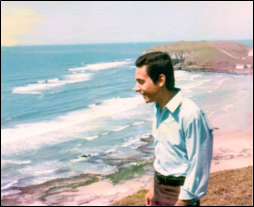
\includegraphics[width=\linewidth]{17/paulo-casamento.png}
\end{subfigure}
\hfill
\begin{subfigure}[h]{0.4\linewidth}
\centering
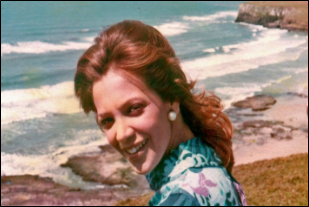
\includegraphics[width=1\linewidth]{17/teresa-casamento.png}
\end{subfigure}
\caption{Paulo e eu, aos vinte e seis anos, quando nos casamos.}
\end{figure}

